\chapter{Introduction to Time Series}
\label{ch:intro_time_series}

% ==============================================================================
% Lecture: 10/08/2026
% ==============================================================================
\section{Time Series Definition \& Decomposition Models}
\lecturedate{10/08/2026}

\begin{definition}{Time Series}{time_series_def}
A \textbf{Time Series} is data which is collected over a period of time and arranged in a chronological order.
\end{definition}

\subsection{Components of Time Series}
A time series $Y$ consists of four primary components:
\begin{itemize}[leftmargin=*]
    \item $\bm{T} \rightarrow$ \textbf{Trend:} Long-term progression or general direction in the data.
    \item $\bm{S} \rightarrow$ \textbf{Seasonality:} Short-term periodic fluctuations repeating at regular intervals.
    \item $\bm{C} \rightarrow$ \textbf{Cyclical:} Wavelike oscillations over longer durations (business/economic cycles).
    \item $\bm{I} \rightarrow$ \textbf{Irregular Component:} Random, unpredictable variations or noise.
\end{itemize}

\subsection{Decomposition Models}
The relationship among the four components is represented as:

\begin{formulabox}[Decomposition Formulations]
\begin{enumerate}[leftmargin=*]
    \item \textbf{Additive Model:}
    \begin{equation}
        Y = T + S + C + I
    \end{equation}
    
    \item \textbf{Multiplicative Model:}
    \begin{equation}
        Y = T \times S \times C \times I
    \end{equation}
\end{enumerate}
\end{formulabox}

\begin{remarkbox}[Logarithmic Transformation]
Applying the natural logarithm transforms a multiplicative model into an additive form:
\begin{equation}
    Y = S \cdot C \cdot T \cdot I \implies \ln(Y) = \ln(S) + \ln(C) + \ln(T) + \ln(I)
\end{equation}
\end{remarkbox}

% ==============================================================================
% Lecture: 13/08/2026
% ==============================================================================
\section{Time Series Analysis \& Forecasting Fundamentals}
\lecturedate{13/08/2026}

\subsection{Classification of Data}
In time series analysis and forecasting, data is broadly categorized into:

\begin{center}
\begin{tikzpicture}[
    node distance=1.2cm and 2.5cm,
    box/.style={rectangle, draw=navyblue, fill=lightgraybg, rounded corners=2pt, minimum width=2.5cm, minimum height=0.8cm, font=\bfseries\sffamily\small, align=center},
    arrow/.style={thick, ->, >=stealth, color=navyblue}
]
    % Root Node
    \node[box] (data) {Data};
    
    % Branches
    \node[box, below left=of data] (qual) {Qualitative};
    \node[box, below right=of data] (quant) {Quantitative};
    
    % Connections
    \draw[arrow] (data) -- (qual);
    \draw[arrow] (data) -- (quant);
\end{tikzpicture}
\end{center}

\subsection{Types of Data}
Based on observation structures:
\begin{enumerate}[leftmargin=*]
    \item \textbf{Time Series Data}
    \item \textbf{Cross-Sectional Data}
    \item \textbf{Panel Data}
\end{enumerate}

\subsection{Benefits of Time Series}
General benefits include understanding past behaviors, modeling underlying dynamics, forecasting future outcomes, and supporting operational planning.

% ==============================================================================
% Lecture: 17/08/2026
% ==============================================================================
\section{Data Notations, Analytical Uses \& Forecasting Taxonomy}
\lecturedate{17/08/2026}

\subsection{Mathematical Representation of Data Types}
Depending on the dimensional index of observation:
\begin{itemize}[leftmargin=*]
    \item \textbf{Time Series (TS):} Observations indexed chronologically over time $t$:
    \begin{equation}
        \text{TS} = y_t
    \end{equation}
    \item \textbf{Cross-Sectional (CS):} Observations across multiple individual entities $i$ at a single point in time:
    \begin{equation}
        \text{CS} = y_i
    \end{equation}
    \item \textbf{Panel Data (P):} Observations across both entities $i$ and time periods $t$:
    \begin{equation}
        \text{P} = y_{it}
    \end{equation}
\end{itemize}

\begin{example}{Time Series Sales Realization}{ts_sales_table}
An illustration of a univariate time series showing sales ($y_t$) over time periods $t = 1, 2, \dots, 7$:
\begin{center}
\small
\begin{tabular}{|c|c|}
\hline
\textbf{Time ($t$)} & \textbf{Sales ($y_t$)} \\
\hline
1 & 20 \\
2 & 16 \\
3 & 12 \\
4 & 8  \\
5 & 4  \\
6 & 0  \\
7 & $-4$ \\
\hline
\end{tabular}
\end{center}
\end{example}

\subsection{Analytical Uses \& Benefits}
\begin{itemize}[leftmargin=*]
    \item \textbf{Descriptive (Time Series):} Describing and tracking temporal movements.
    \item \textbf{Spatial (Cross-Sectional):} Evaluating spatial variations across entities.
    \item \textbf{Explorative:} Analyzing relationships and interactions between two or more variables.
\end{itemize}

\subsection{Key Application Areas}
\begin{enumerate}[leftmargin=*, noitemsep]
    \item \textbf{Economic:} Macroeconomic trends, inflation, growth indices.
    \item \textbf{Sales:} Revenue forecasting, sales volume trajectories.
    \item \textbf{Performance:} Operational efficiency, financial asset returns.
    \item \textbf{Portfolio:} Asset allocation, risk-return profiling.
    \item \textbf{Demand:} Consumer demand estimation, inventory planning.
    \item \textbf{Yield:} Bond yields, interest rates, agricultural outputs.
\end{enumerate}

\subsection{Forecasting Approaches \& Horizons}
\begin{itemize}[leftmargin=*]
    \item \textbf{Approaches to Forecasting:}
    \begin{itemize}[noitemsep]
        \item \textit{Quantitative:} Model-based statistical methods on historical numerical series.
        \item \textit{Qualitative:} Intuition, expert judgment, and opinion gathering.
        \item \textit{Combination (Team / Consensus):} Synthesizing multiple quantitative and qualitative models.
    \end{itemize}
    
    \item \textbf{Forecasting Horizons (Types):}
    \begin{itemize}[noitemsep]
        \item \textbf{Short Term (ST):} Immediate horizon / up to 3 months.
        \item \textbf{Medium Term (MT):} 3 to 6 months / 1 year.
        \item \textbf{Long Term (LT):} Extended planning horizons (5+ years).
    \end{itemize}
\end{itemize}

\newpage
\begin{landscape}
\thispagestyle{empty}
\vspace*{-0.5cm}
\noindent{\large\textbf{1.3.5 \quad Comprehensive Taxonomy of Forecasting Methodologies}}\\[0.2cm]
\begin{center}
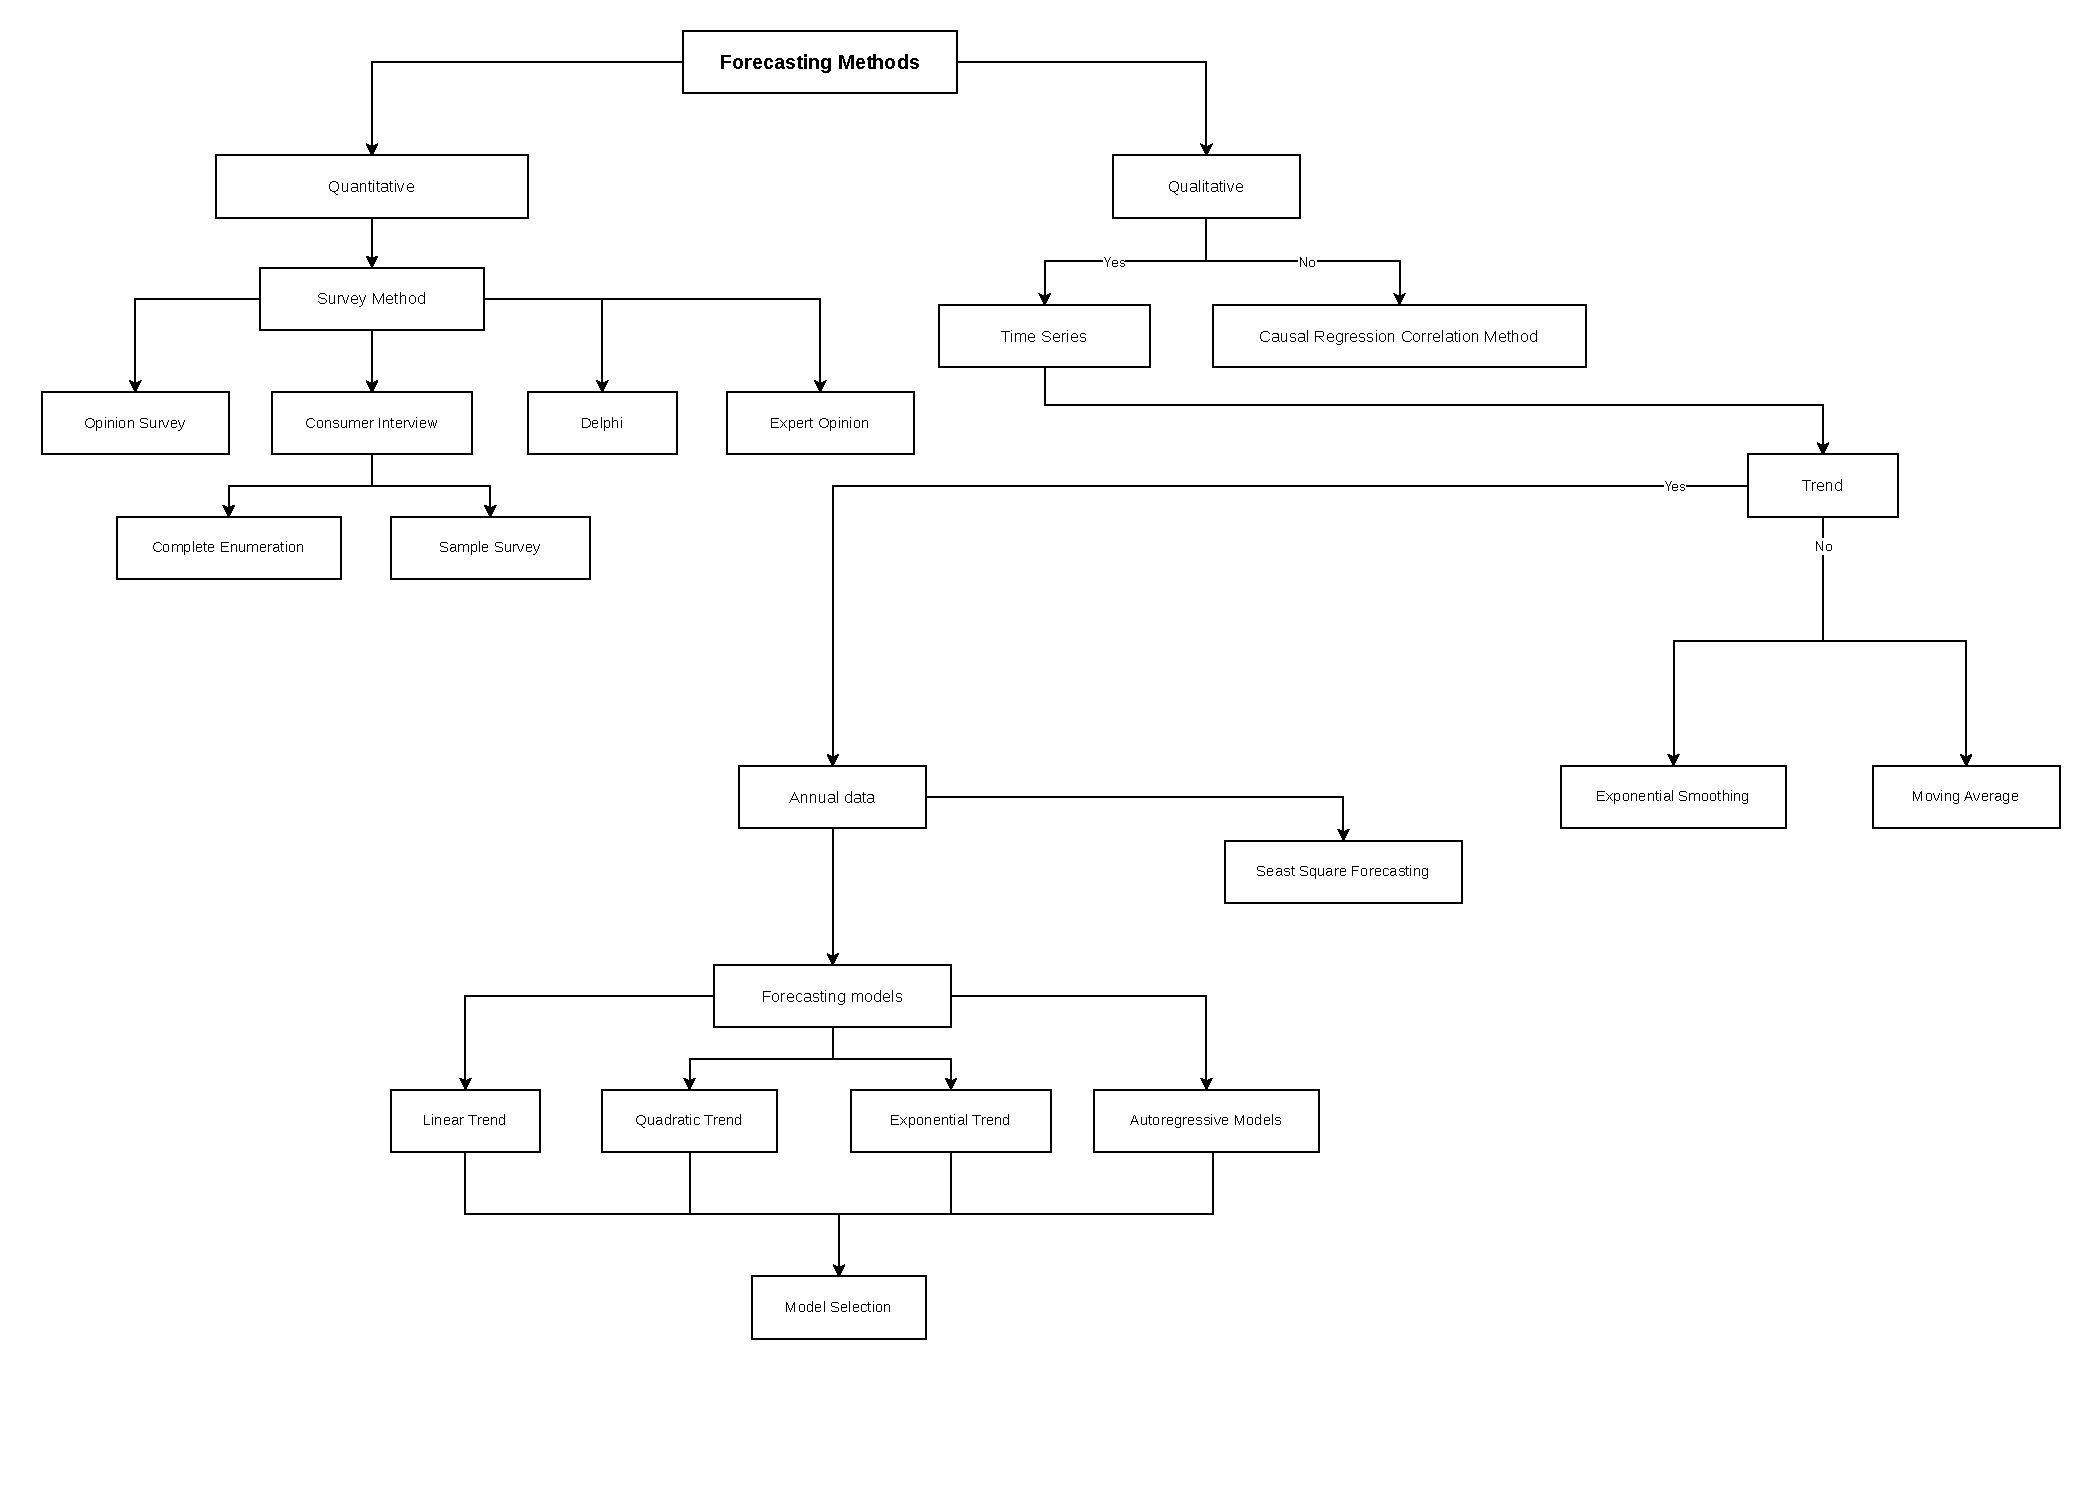
\includegraphics[width=1.02\linewidth, height=0.90\textheight, keepaspectratio]{figures/forecasting_methods_flowchart.pdf}
\end{center}
\end{landscape}

\subsection{Trend Models for Annual Data}
For annual time series exhibiting long-term movement, trend equations are specified and estimated via least squares or autoregression before model selection:

\begin{formulabox}[Summary of Trend Models]
\begin{enumerate}[leftmargin=*]
    \item \textbf{Linear Trend:}
    \begin{equation}
        Y_t = \beta_0 + \beta_1 t + \varepsilon_t
    \end{equation}
    \item \textbf{Quadratic (Curvilinear) Trend:}
    \begin{equation}
        Y_t = \beta_0 + \beta_1 t + \beta_2 t^2 + \varepsilon_t
    \end{equation}
    \item \textbf{Exponential Trend:}
    \begin{equation}
        Y_t = \beta_0 e^{\beta_1 t} \cdot \varepsilon_t \iff \ln(Y_t) = \ln(\beta_0) + \beta_1 t + \ln(\varepsilon_t)
    \end{equation}
    \item \textbf{Autoregressive Trend Model ($\AR(p)$):}
    \begin{equation}
        Y_t = c + \phi_1 Y_{t-1} + \dots + \phi_p Y_{t-p} + \varepsilon_t
    \end{equation}
\end{enumerate}
\end{formulabox}
